% !TEX TS-program = pdflatex
% !TEX encoding = UTF-8 Unicode

% This is a simple template for a LaTeX document using the "article" class.
% See "book", "report", "letter" for other types of document.

\documentclass[11pt]{article}\usepackage[]{graphicx}\usepackage[]{color}
%% maxwidth is the original width if it is less than linewidth
%% otherwise use linewidth (to make sure the graphics do not exceed the margin)
\makeatletter
\def\maxwidth{ %
  \ifdim\Gin@nat@width>\linewidth
    \linewidth
  \else
    \Gin@nat@width
  \fi
}
\makeatother

\definecolor{fgcolor}{rgb}{0.345, 0.345, 0.345}
\newcommand{\hlnum}[1]{\textcolor[rgb]{0.686,0.059,0.569}{#1}}%
\newcommand{\hlstr}[1]{\textcolor[rgb]{0.192,0.494,0.8}{#1}}%
\newcommand{\hlcom}[1]{\textcolor[rgb]{0.678,0.584,0.686}{\textit{#1}}}%
\newcommand{\hlopt}[1]{\textcolor[rgb]{0,0,0}{#1}}%
\newcommand{\hlstd}[1]{\textcolor[rgb]{0.345,0.345,0.345}{#1}}%
\newcommand{\hlkwa}[1]{\textcolor[rgb]{0.161,0.373,0.58}{\textbf{#1}}}%
\newcommand{\hlkwb}[1]{\textcolor[rgb]{0.69,0.353,0.396}{#1}}%
\newcommand{\hlkwc}[1]{\textcolor[rgb]{0.333,0.667,0.333}{#1}}%
\newcommand{\hlkwd}[1]{\textcolor[rgb]{0.737,0.353,0.396}{\textbf{#1}}}%

\usepackage{framed}
\makeatletter
\newenvironment{kframe}{%
 \def\at@end@of@kframe{}%
 \ifinner\ifhmode%
  \def\at@end@of@kframe{\end{minipage}}%
  \begin{minipage}{\columnwidth}%
 \fi\fi%
 \def\FrameCommand##1{\hskip\@totalleftmargin \hskip-\fboxsep
 \colorbox{shadecolor}{##1}\hskip-\fboxsep
     % There is no \\@totalrightmargin, so:
     \hskip-\linewidth \hskip-\@totalleftmargin \hskip\columnwidth}%
 \MakeFramed {\advance\hsize-\width
   \@totalleftmargin\z@ \linewidth\hsize
   \@setminipage}}%
 {\par\unskip\endMakeFramed%
 \at@end@of@kframe}
\makeatother

\definecolor{shadecolor}{rgb}{.97, .97, .97}
\definecolor{messagecolor}{rgb}{0, 0, 0}
\definecolor{warningcolor}{rgb}{1, 0, 1}
\definecolor{errorcolor}{rgb}{1, 0, 0}
\newenvironment{knitrout}{}{} % an empty environment to be redefined in TeX

\usepackage{alltt} % use larger type; default would be 10pt

\usepackage[utf8]{inputenc} % set input encoding (not needed with XeLaTeX)

%%% Examples of Article customizations
% These packages are optional, depending whether you want the features they provide.
% See the LaTeX Companion or other references for full information.

%%% PAGE DIMENSIONS
\usepackage{geometry} % to change the page dimensions
\geometry{a4paper} % or letterpaper (US) or a5paper or....
% \geometry{margin=2in} % for example, change the margins to 2 inches all round
% \geometry{landscape} % set up the page for landscape
%   read geometry.pdf for detailed page layout information

\usepackage{graphicx} % support the \includegraphics command and options

% \usepackage[parfill]{parskip} % Activate to begin paragraphs with an empty line rather than an indent

%%% PACKAGES
\usepackage{booktabs} % for much better looking tables
\usepackage{array} % for better arrays (eg matrices) in maths
\usepackage{paralist} % very flexible & customisable lists (eg. enumerate/itemize, etc.)
\usepackage{verbatim} % adds environment for commenting out blocks of text & for better verbatim
\usepackage{subfig} % make it possible to include more than one captioned figure/table in a single float
% These packages are all incorporated in the memoir class to one degree or another...

%%% HEADERS & FOOTERS
\usepackage{fancyhdr} % This should be set AFTER setting up the page geometry
\pagestyle{fancy} % options: empty , plain , fancy
\renewcommand{\headrulewidth}{0pt} % customise the layout...
\lhead{}\chead{}\rhead{}
\lfoot{}\cfoot{\thepage}\rfoot{}

%%% SECTION TITLE APPEARANCE
\usepackage{sectsty}
\allsectionsfont{\sffamily\mdseries\upshape} % (See the fntguide.pdf for font help)
% (This matches ConTeXt defaults)

%%% ToC (table of contents) APPEARANCE
\usepackage[nottoc,notlof,notlot]{tocbibind} % Put the bibliography in the ToC
\usepackage[titles,subfigure]{tocloft} % Alter the style of the Table of Contents
\renewcommand{\cftsecfont}{\rmfamily\mdseries\upshape}
\renewcommand{\cftsecpagefont}{\rmfamily\mdseries\upshape} % No bold!
\usepackage{tipa}
\usepackage{natbib}
%%% END Article customizations

%%% The "real" document content comes below...

\title{Brief Article}
\author{The Author}
%\date{} % Activate to display a given date or no date (if empty),
         % otherwise the current date is printed 



\IfFileExists{upquote.sty}{\usepackage{upquote}}{}
\begin{document}
\begin{center}
530 Analysis and Results

Michael McAuliffe
\end{center}

\section{Analysis}

This section outlines more the analysis details (nitty-gritty R code and summary outputs), and should probably primarily be used as a reference when reading the Results section below, which is a copy-paste from its current form in my dissertation.  The R code is generated using knitr with the lme4 code commented (so that it doesn't actually run in real time when generating the code).

Experimental manipulations are in the columns Attention and ExposureType.  Attention has two levels ('attend' and 'noattend') where 'attend' participants were given additional instructions about the speaker's ambiguous /s/ sound.  ExposureType is different between Experiments 1/2 and Experiment 3.  In Experiments 1 and 2, it has the levels 'initial' and 'final' which refer to which syllable the ambiguous /s/ sound is embedded in.  In Experiment 3, it has the levels 'predictive' and 'unpredictive', referring to whether the sentence preceding the word is predictive of the word the ambiguous /s/ sound is embedded in.  In Experiment 3, all ambiguous /s/ sounds are in 'final' words taken from Experiments 1.

Predictions, I suppose, would be that participants in the 'final' condition should show more perceptual learning than participants in the 'initial' condition, due to the increased lexical bias in the 'final' stimuli.  Participants in the 'noattend' condition should show greater perceptual learning effects than participants in the 'attend' condition, because the instructions are worded in such a way to warn participants to be careful that they make the correct choice between word and nonword in exposure.

In Experiment 3, predictions would be that participants in the 'predictive' condition should show greater perceptual learning than participants and in the 'unpredictive' condition, since semantic predictability has been shown to behave like lexical bias in phoneme categorization tasks.  If the effects of lexical bias and semantic predictability are additive, they should show more perceptual learning than those in Experiment 1 (which uses the same word types for embedding ambiguous tokens in).  The effect of attention should be much the same, since the instructions are identical, and the task is no harder (or shouldn't require any more attention) than the lexical decision task.

Additionally, there's an attentional gradience hypothesis being tested.  If attention/attentional resources has a gradient, modulatory effect on linguistic factors, then we shouldn't see much of an interaction between attention and exposure type.  Increased lexical bias should lead to greater perceptual learning, and attention should result in less perceptual learning, and so a gradient pattern across the four conditions should be present.  On the other hand, if attention is more all-or-nothing, then we might expect to see an interaction between attention and the linguistic factors, with attention overriding any effect of linguistic factors on perceptual learning.  This would lead to a pattern across conditions where all attention conditions (and perhaps attention-drawing conditions, like 'initial' instead of 'final') have the same perceptual learning with some outliers for the non-attention, non-attention-getting conditions ('noattend', 'final').

\subsection{Exposure}

The exposure data analyzed was a subset of the original data, where nonword trials were excluded.  Additional exclusions were that reaction times were greater than 200 ms and less than 2500 ms.  Non responses were also omited.

\begin{knitrout}\footnotesize
\definecolor{shadecolor}{rgb}{0.969, 0.969, 0.969}\color{fgcolor}\begin{kframe}
\begin{alltt}
 \hlstd{expose} \hlkwb{<-} \hlkwd{na.omit}\hlstd{(expose)}
 \hlstd{expose} \hlkwb{<-} \hlkwd{subset}\hlstd{(expose,RT} \hlopt{>} \hlnum{200} \hlopt{&} \hlstd{RT} \hlopt{<} \hlnum{2500}\hlstd{)}
 \hlstd{expose.word} \hlkwb{<-} \hlkwd{subset}\hlstd{(expose,Lexicality}\hlopt{==}\hlstr{'Word'}\hlstd{)}
\end{alltt}
\end{kframe}
\end{knitrout}

Reaction time was transformed into cLogRT by taking the logarithm of RT and subtracting the mean:

\begin{knitrout}\footnotesize
\definecolor{shadecolor}{rgb}{0.969, 0.969, 0.969}\color{fgcolor}\begin{kframe}
\begin{alltt}
 \hlstd{expose.word}\hlopt{$}\hlstd{LogRT} \hlkwb{<-} \hlkwd{log}\hlstd{(expose.word}\hlopt{$}\hlstd{RT)}
 \hlstd{expose.word}\hlopt{$}\hlstd{cLogRT} \hlkwb{<-} \hlstd{expose.word}\hlopt{$}\hlstd{LogRT} \hlopt{-} \hlkwd{mean}\hlstd{(expose.word}\hlopt{$}\hlstd{LogRT)}
\end{alltt}
\end{kframe}
\end{knitrout}

The resulting data frame had the following structure.

\begin{knitrout}\footnotesize
\definecolor{shadecolor}{rgb}{0.969, 0.969, 0.969}\color{fgcolor}\begin{kframe}
\begin{alltt}
 \hlkwd{summary}\hlstd{(expose.word[,}\hlkwd{c}\hlstd{(}\hlstr{'Subject'}\hlstd{,} \hlstr{'Word'}\hlstd{,} \hlstr{'Experiment'}\hlstd{,} \hlstr{'Attention'}\hlstd{,}
 \hlstr{'ExposureType'}\hlstd{,} \hlstr{'itemtype2'}\hlstd{,} \hlstr{'Trial'}\hlstd{,} \hlstr{'RT'}\hlstd{,} \hlstr{'cLogRT'}\hlstd{,} \hlstr{'ACC'}\hlstd{)])}
\end{alltt}
\begin{verbatim}
##     Subject            Word       Experiment     Attention   
##  ns1-101:  100   acorn   :  186   exp1:9318   noattend:9393  
##  ns1-106:  100   cabin   :  186   exp2:9105   attend  :9030  
##  ns1-108:  100   calendar:  186                              
##  ns1-114:  100   campfire:  186                              
##  ns1-117:  100   candy   :  186                              
##  ns1-120:  100   cowboy  :  186                              
##  (Other):17823   (Other) :17307                              
##   ExposureType   itemtype2         Trial             RT      
##  initial:9284   Filler:11073   Min.   :  1.0   Min.   : 204  
##  final  :9139   S     : 3649   1st Qu.: 53.0   1st Qu.: 835  
##                 SH    : 3701   Median :104.0   Median : 956  
##                                Mean   :102.7   Mean   :1026  
##                                3rd Qu.:153.0   3rd Qu.:1130  
##                                Max.   :200.0   Max.   :2495  
##                                                              
##      cLogRT              ACC        
##  Min.   :-1.58170   Min.   :0.0000  
##  1st Qu.:-0.17239   1st Qu.:1.0000  
##  Median :-0.03707   Median :1.0000  
##  Mean   : 0.00000   Mean   :0.8974  
##  3rd Qu.: 0.13015   3rd Qu.:1.0000  
##  Max.   : 0.92222   Max.   :1.0000  
## 
\end{verbatim}
\end{kframe}
\end{knitrout}

Two models were fit for this data per experiment ('exp2' actually refers to Experiment 1 in the dissertation), one with ACC as a dependent measure:

\begin{knitrout}\footnotesize
\definecolor{shadecolor}{rgb}{0.969, 0.969, 0.969}\color{fgcolor}\begin{kframe}
\begin{alltt}
 \hlcom{#experiment.1.expose.mod.randslope <- }
 \hlcom{#glmer(ACC ~ itemtype2*Attention*ExposureType }
 \hlcom{#+ (1+itemtype2|Subject) + (1+Attention|Word),}
 \hlcom{#family='binomial', }
 \hlcom{#data = subset(expose.word, Experiment=='exp2'),}
 \hlcom{#control = glmerControl(optCtrl=list(maxfun=200000) ))}
 \hlkwd{summary}\hlstd{(experiment.1.expose.mod.randslope)}
\end{alltt}
\begin{verbatim}
## Generalized linear mixed model fit by maximum likelihood (Laplace
##   Approximation) [glmerMod]
##  Family: binomial  ( logit )
## Formula: ACC ~ itemtype2 * Attention * ExposureType + (1 + itemtype2 |  
##     Subject) + (1 + Attention | Word)
##    Data: subset(expose.word, Experiment == "exp2")
## Control: glmerControl(optCtrl = list(maxfun = 2e+05))
## 
##      AIC      BIC   logLik deviance df.resid 
##   4058.4   4207.8  -2008.2   4016.4     9084 
## 
## Scaled residuals: 
##      Min       1Q   Median       3Q      Max 
## -11.5890   0.0966   0.1478   0.2359  11.7658 
## 
## Random effects:
##  Groups  Name            Variance Std.Dev. Corr       
##  Word    (Intercept)     1.130175 1.0631              
##          Attentionattend 0.009255 0.0962   1.00       
##  Subject (Intercept)     1.148901 1.0719              
##          itemtype2S      2.127599 1.4586   -0.39      
##          itemtype2SH     0.652830 0.8080   -0.27  0.36
## Number of obs: 9105, groups:  Word, 120; Subject, 92
## 
## Fixed effects:
##                                               Estimate Std. Error z value
## (Intercept)                                     3.3798     0.2971  11.375
## itemtype2S                                     -1.7852     0.4547  -3.927
## itemtype2SH                                     0.2295     0.4276   0.537
## Attentionattend                                 0.7134     0.3785   1.885
## ExposureTypefinal                               0.6434     0.3750   1.716
## itemtype2S:Attentionattend                     -0.5231     0.5152  -1.015
## itemtype2SH:Attentionattend                    -0.4271     0.4354  -0.981
## itemtype2S:ExposureTypefinal                   -0.1331     0.6206  -0.214
## itemtype2SH:ExposureTypefinal                  -0.6232     0.4317  -1.444
## Attentionattend:ExposureTypefinal              -0.6163     0.5347  -1.152
## itemtype2S:Attentionattend:ExposureTypefinal   -0.1106     0.7352  -0.150
## itemtype2SH:Attentionattend:ExposureTypefinal   0.1954     0.6111   0.320
##                                               Pr(>|z|)    
## (Intercept)                                    < 2e-16 ***
## itemtype2S                                    8.62e-05 ***
## itemtype2SH                                     0.5914    
## Attentionattend                                 0.0594 .  
## ExposureTypefinal                               0.0862 .  
## itemtype2S:Attentionattend                      0.3100    
## itemtype2SH:Attentionattend                     0.3267    
## itemtype2S:ExposureTypefinal                    0.8302    
## itemtype2SH:ExposureTypefinal                   0.1489    
## Attentionattend:ExposureTypefinal               0.2491    
## itemtype2S:Attentionattend:ExposureTypefinal    0.8804    
## itemtype2SH:Attentionattend:ExposureTypefinal   0.7491    
## ---
## Signif. codes:  0 '***' 0.001 '**' 0.01 '*' 0.05 '.' 0.1 ' ' 1
## 
## Correlation of Fixed Effects:
##             (Intr) itmt2S itm2SH Attntn ExpsrT it2S:A it2SH:A i2S:ET
## itemtype2S  -0.483                                                  
## itemtype2SH -0.366  0.284                                           
## Attentnttnd -0.571  0.238  0.130                                    
## ExpsrTypfnl -0.574  0.244  0.158  0.452                             
## itmtyp2S:At  0.268 -0.508 -0.136 -0.490 -0.217                      
## itmtyp2SH:A  0.167 -0.153 -0.441 -0.328 -0.158  0.321               
## itmtyp2S:ET  0.228 -0.648 -0.126 -0.181 -0.402  0.378  0.124        
## itmty2SH:ET  0.195 -0.170 -0.490 -0.154 -0.364  0.151  0.476   0.285
## Attntntt:ET  0.400 -0.169 -0.110 -0.676 -0.701  0.330  0.246   0.282
## itmt2S:A:ET -0.190  0.358  0.106  0.329  0.339 -0.693 -0.231  -0.569
## itm2SH:A:ET -0.135  0.119  0.335  0.242  0.257 -0.233 -0.703  -0.200
##             i2SH:E Att:ET i2S:A:
## itemtype2S                      
## itemtype2SH                     
## Attentnttnd                     
## ExpsrTypfnl                     
## itmtyp2S:At                     
## itmtyp2SH:A                     
## itmtyp2S:ET                     
## itmty2SH:ET                     
## Attntntt:ET  0.255              
## itmt2S:A:ET -0.240 -0.488       
## itm2SH:A:ET -0.704 -0.376  0.350
\end{verbatim}
\end{kframe}
\end{knitrout}

And one with cLogRT:

\begin{knitrout}\footnotesize
\definecolor{shadecolor}{rgb}{0.969, 0.969, 0.969}\color{fgcolor}\begin{kframe}
\begin{alltt}
 \hlcom{#experiment.1.expose.mod.rt <- }
 \hlcom{#lmer(cLogRT ~ itemtype2*Attention*ExposureType }
 \hlcom{#+ (1+itemtype2|Subject) + (1+Attention|Word),}
 \hlcom{#data = subset(expose.word, Experiment == 'exp2'), }
 \hlcom{#control = lmerControl(optCtrl = list(maxfun = 200000) ))}
 \hlkwd{summary}\hlstd{(experiment.1.expose.mod.rt)}
\end{alltt}
\begin{verbatim}
## Linear mixed model fit by REML ['lmerMod']
## Formula: cLogRT ~ itemtype2 * Attention * ExposureType + (1 + itemtype2 |  
##     Subject) + (1 + Attention | Word)
##    Data: subset(expose.word, Experiment == "exp2")
## Control: lmerControl(optCtrl = list(maxfun = 2e+05))
## 
## REML criterion at convergence: -2390.9
## 
## Scaled residuals: 
##     Min      1Q  Median      3Q     Max 
## -6.6999 -0.6209 -0.1493  0.4321  5.5068 
## 
## Random effects:
##  Groups   Name            Variance  Std.Dev. Corr       
##  Word     (Intercept)     4.739e-03 0.068844            
##           Attentionattend 2.263e-04 0.015042 0.19       
##  Subject  (Intercept)     1.068e-02 0.103343            
##           itemtype2S      3.403e-03 0.058334  0.19      
##           itemtype2SH     1.286e-05 0.003586  0.79 -0.45
##  Residual                 4.160e-02 0.203972            
## Number of obs: 9105, groups:  Word, 120; Subject, 92
## 
## Fixed effects:
##                                                 Estimate Std. Error
## (Intercept)                                   -0.0434562  0.0235274
## itemtype2S                                     0.1578882  0.0240035
## itemtype2SH                                    0.0344607  0.0208198
## Attentionattend                               -0.0323302  0.0311912
## ExposureTypefinal                             -0.0156962  0.0314938
## itemtype2S:Attentionattend                     0.0346502  0.0233588
## itemtype2SH:Attentionattend                    0.0091988  0.0159445
## itemtype2S:ExposureTypefinal                  -0.0194982  0.0318771
## itemtype2SH:ExposureTypefinal                 -0.0248743  0.0156440
## Attentionattend:ExposureTypefinal              0.0294098  0.0445085
## itemtype2S:Attentionattend:ExposureTypefinal   0.0002751  0.0332488
## itemtype2SH:Attentionattend:ExposureTypefinal  0.0076472  0.0221003
##                                               t value
## (Intercept)                                    -1.847
## itemtype2S                                      6.578
## itemtype2SH                                     1.655
## Attentionattend                                -1.037
## ExposureTypefinal                              -0.498
## itemtype2S:Attentionattend                      1.483
## itemtype2SH:Attentionattend                     0.577
## itemtype2S:ExposureTypefinal                   -0.612
## itemtype2SH:ExposureTypefinal                  -1.590
## Attentionattend:ExposureTypefinal               0.661
## itemtype2S:Attentionattend:ExposureTypefinal    0.008
## itemtype2SH:Attentionattend:ExposureTypefinal   0.346
## 
## Correlation of Fixed Effects:
##             (Intr) itmt2S itm2SH Attntn ExpsrT it2S:A it2SH:A i2S:ET
## itemtype2S  -0.110                                                  
## itemtype2SH -0.197  0.209                                           
## Attentnttnd -0.642 -0.027  0.022                                    
## ExpsrTypfnl -0.640 -0.022  0.026  0.483                             
## itmtyp2S:At -0.037 -0.441 -0.046  0.043  0.023                      
## itmtyp2SH:A  0.037 -0.058 -0.315 -0.077 -0.034  0.149               
## itmtyp2S:ET -0.023 -0.650 -0.039  0.017  0.036  0.336  0.050        
## itmty2SH:ET  0.047 -0.068 -0.361 -0.035 -0.073  0.070  0.471   0.107
## Attntntt:ET  0.453  0.016 -0.019 -0.698 -0.708 -0.034  0.049  -0.025
## itmt2S:A:ET  0.022  0.314  0.037 -0.034 -0.034 -0.698 -0.098  -0.493
## itm2SH:A:ET -0.033  0.048  0.255  0.050  0.051 -0.100 -0.679  -0.076
##             i2SH:E Att:ET i2S:A:
## itemtype2S                      
## itemtype2SH                     
## Attentnttnd                     
## ExpsrTypfnl                     
## itmtyp2S:At                     
## itmtyp2SH:A                     
## itmtyp2S:ET                     
## itmty2SH:ET                     
## Attntntt:ET  0.051              
## itmt2S:A:ET -0.102  0.049       
## itm2SH:A:ET -0.708 -0.072  0.144
\end{verbatim}
\end{kframe}
\end{knitrout}

For Experiment 2, the same specifications were used, ACC:

\begin{knitrout}\footnotesize
\definecolor{shadecolor}{rgb}{0.969, 0.969, 0.969}\color{fgcolor}\begin{kframe}
\begin{alltt}
 \hlcom{#experiment.2.expose.mod.randslope <- }
 \hlcom{#glmer(ACC ~ itemtype2*Attention*ExposureType }
 \hlcom{#+ (1+itemtype2|Subject) + (1+Attention|Word),}
 \hlcom{#family='binomial',}
 \hlcom{#data = subset(expose.word, Experiment == 'exp1'),}
 \hlcom{#control = glmerControl(optCtrl = list(maxfun = 200000) ))}
  \hlkwd{summary}\hlstd{(experiment.2.expose.mod.randslope)}
\end{alltt}
\begin{verbatim}
## Generalized linear mixed model fit by maximum likelihood (Laplace
##   Approximation) [glmerMod]
##  Family: binomial  ( logit )
## Formula: ACC ~ itemtype2 * Attention * ExposureType + (1 + itemtype2 |  
##     Subject) + (1 + Attention | Word)
##    Data: subset(expose.word, Experiment == "exp1")
## Control: glmerControl(optCtrl = list(maxfun = 2e+05))
## 
##      AIC      BIC   logLik deviance df.resid 
##   4121.6   4271.6  -2039.8   4079.6     9297 
## 
## Scaled residuals: 
##      Min       1Q   Median       3Q      Max 
## -10.2759   0.0919   0.1304   0.2040   3.7838 
## 
## Random effects:
##  Groups  Name            Variance Std.Dev. Corr       
##  Word    (Intercept)     1.2435   1.1151              
##          Attentionattend 0.1208   0.3476   0.31       
##  Subject (Intercept)     0.2705   0.5201              
##          itemtype2S      1.9461   1.3950    0.14      
##          itemtype2SH     0.3022   0.5497   -0.46  0.41
## Number of obs: 9318, groups:  Word, 120; Subject, 94
## 
## Fixed effects:
##                                               Estimate Std. Error z value
## (Intercept)                                    3.88112    0.24814  15.641
## itemtype2S                                    -3.17929    0.45293  -7.019
## itemtype2SH                                    0.16709    0.45802   0.365
## Attentionattend                                0.05007    0.28312   0.177
## ExposureTypefinal                             -0.03330    0.25393  -0.131
## itemtype2S:Attentionattend                     0.43790    0.51157   0.856
## itemtype2SH:Attentionattend                    0.31794    0.46820   0.679
## itemtype2S:ExposureTypefinal                  -0.64628    0.59613  -1.084
## itemtype2SH:ExposureTypefinal                  0.14941    0.42008   0.356
## Attentionattend:ExposureTypefinal              0.23077    0.37007   0.624
## itemtype2S:Attentionattend:ExposureTypefinal  -0.48762    0.70961  -0.687
## itemtype2SH:Attentionattend:ExposureTypefinal  0.04503    0.62891   0.072
##                                               Pr(>|z|)    
## (Intercept)                                    < 2e-16 ***
## itemtype2S                                    2.23e-12 ***
## itemtype2SH                                      0.715    
## Attentionattend                                  0.860    
## ExposureTypefinal                                0.896    
## itemtype2S:Attentionattend                       0.392    
## itemtype2SH:Attentionattend                      0.497    
## itemtype2S:ExposureTypefinal                     0.278    
## itemtype2SH:ExposureTypefinal                    0.722    
## Attentionattend:ExposureTypefinal                0.533    
## itemtype2S:Attentionattend:ExposureTypefinal     0.492    
## itemtype2SH:Attentionattend:ExposureTypefinal    0.943    
## ---
## Signif. codes:  0 '***' 0.001 '**' 0.01 '*' 0.05 '.' 0.1 ' ' 1
## 
## Correlation of Fixed Effects:
##             (Intr) itmt2S itm2SH Attntn ExpsrT it2S:A it2SH:A i2S:ET
## itemtype2S  -0.411                                                  
## itemtype2SH -0.440  0.279                                           
## Attentnttnd -0.484  0.145  0.165                                    
## ExpsrTypfnl -0.510  0.150  0.227  0.443                             
## itmtyp2S:At  0.144 -0.467 -0.126 -0.318 -0.131                      
## itmtyp2SH:A  0.181 -0.137 -0.366 -0.375 -0.220  0.284               
## itmtyp2S:ET  0.113 -0.652 -0.126 -0.098 -0.226  0.350  0.122        
## itmty2SH:ET  0.254 -0.178 -0.429 -0.221 -0.495  0.156  0.431   0.271
## Attntntt:ET  0.355 -0.106 -0.159 -0.639 -0.686  0.186  0.318   0.155
## itmt2S:A:ET -0.096  0.334  0.107  0.165  0.190 -0.691 -0.220  -0.515
## itm2SH:A:ET -0.174  0.121  0.296  0.312  0.331 -0.221 -0.628  -0.181
##             i2SH:E Att:ET i2S:A:
## itemtype2S                      
## itemtype2SH                     
## Attentnttnd                     
## ExpsrTypfnl                     
## itmtyp2S:At                     
## itmtyp2SH:A                     
## itmtyp2S:ET                     
## itmty2SH:ET                     
## Attntntt:ET  0.340              
## itmt2S:A:ET -0.228 -0.281       
## itm2SH:A:ET -0.667 -0.484  0.323
\end{verbatim}
\end{kframe}
\end{knitrout}

And cLogRT:

\begin{knitrout}\footnotesize
\definecolor{shadecolor}{rgb}{0.969, 0.969, 0.969}\color{fgcolor}\begin{kframe}
\begin{alltt}
 \hlcom{#experiment.2.expose.mod.rt <- }
 \hlcom{#lmer(cLogRT ~ itemtype2*Attention*ExposureType }
 \hlcom{#+ (1+itemtype2|Subject) + (1+Attention|Word),}
 \hlcom{#data = subset(expose.word, Experiment == 'exp1'), }
 \hlcom{#control = lmerControl(optCtrl = list(maxfun = 200000) ))}
 \hlkwd{summary}\hlstd{(experiment.2.expose.mod.rt)}
\end{alltt}
\begin{verbatim}
## Linear mixed model fit by REML ['lmerMod']
## Formula: cLogRT ~ itemtype2 * Attention * ExposureType + (1 + itemtype2 |  
##     Subject) + (1 + Attention | Word)
##    Data: subset(expose.word, Experiment == "exp1")
## Control: lmerControl(optCtrl = list(maxfun = 2e+05))
## 
## REML criterion at convergence: -2664.3
## 
## Scaled residuals: 
##     Min      1Q  Median      3Q     Max 
## -4.4032 -0.6350 -0.1584  0.4340  4.9672 
## 
## Random effects:
##  Groups   Name            Variance  Std.Dev. Corr       
##  Word     (Intercept)     4.877e-03 0.069838            
##           Attentionattend 6.169e-04 0.024837 -0.57      
##  Subject  (Intercept)     9.937e-03 0.099686            
##           itemtype2S      5.741e-03 0.075768 -0.12      
##           itemtype2SH     9.433e-05 0.009713  0.53 -0.91
##  Residual                 4.056e-02 0.201391            
## Number of obs: 9318, groups:  Word, 120; Subject, 94
## 
## Fixed effects:
##                                                Estimate Std. Error t value
## (Intercept)                                   -0.019786   0.022495  -0.880
## itemtype2S                                     0.261638   0.025790  10.145
## itemtype2SH                                    0.026851   0.020919   1.284
## Attentionattend                                0.021293   0.030294   0.703
## ExposureTypefinal                             -0.033377   0.029447  -1.133
## itemtype2S:Attentionattend                    -0.019533   0.027751  -0.704
## itemtype2SH:Attentionattend                    0.021734   0.016771   1.296
## itemtype2S:ExposureTypefinal                  -0.024672   0.034369  -0.718
## itemtype2SH:ExposureTypefinal                  0.002162   0.015152   0.143
## Attentionattend:ExposureTypefinal             -0.014044   0.042560  -0.330
## itemtype2S:Attentionattend:ExposureTypefinal  -0.028576   0.038880  -0.735
## itemtype2SH:Attentionattend:ExposureTypefinal -0.026824   0.021900  -1.225
## 
## Correlation of Fixed Effects:
##             (Intr) itmt2S itm2SH Attntn ExpsrT it2S:A it2SH:A i2S:ET
## itemtype2S  -0.249                                                  
## itemtype2SH -0.187  0.152                                           
## Attentnttnd -0.647  0.102  0.036                                    
## ExpsrTypfnl -0.641  0.083  0.011  0.476                             
## itmtyp2S:At  0.127 -0.567 -0.029 -0.172 -0.077                      
## itmtyp2SH:A  0.061 -0.039 -0.507 -0.049 -0.014  0.025               
## itmtyp2S:ET  0.082 -0.659 -0.001 -0.061 -0.127  0.408  0.001        
## itmty2SH:ET  0.020 -0.001 -0.355 -0.015 -0.031  0.001  0.443   0.002
## Attntntt:ET  0.444 -0.057 -0.008 -0.704 -0.692  0.114  0.020   0.088
## itmt2S:A:ET -0.072  0.388  0.001  0.114  0.112 -0.704 -0.002  -0.593
## itm2SH:A:ET -0.014  0.001  0.245  0.022  0.021 -0.002 -0.654  -0.002
##             i2SH:E Att:ET i2S:A:
## itemtype2S                      
## itemtype2SH                     
## Attentnttnd                     
## ExpsrTypfnl                     
## itmtyp2S:At                     
## itmtyp2SH:A                     
## itmtyp2S:ET                     
## itmty2SH:ET                     
## Attntntt:ET  0.021              
## itmt2S:A:ET -0.002 -0.162       
## itm2SH:A:ET -0.692 -0.031  0.003
\end{verbatim}
\end{kframe}
\end{knitrout}

Experiment 3 has not really been analyzed, but here's the summary of the exposure data frame for it:

\begin{knitrout}\footnotesize
\definecolor{shadecolor}{rgb}{0.969, 0.969, 0.969}\color{fgcolor}\begin{kframe}
\begin{alltt}
 \hlkwd{summary}\hlstd{(expose3[,}\hlkwd{c}\hlstd{(}\hlstr{'Subject'}\hlstd{,} \hlstr{'Word'}\hlstd{,} \hlstr{'Distractor'}\hlstd{,}
 \hlstr{'Predictability'}\hlstd{,} \hlstr{'Attention'}\hlstd{,} \hlstr{'Type'}\hlstd{,} \hlstr{'RT'}\hlstd{,} \hlstr{'ACC'}\hlstd{,} \hlstr{'Sentence'}\hlstd{)])}
\end{alltt}
\begin{verbatim}
##     Subject          Word          Distractor        Predictability
##  ns3-104: 100   acorn  :  43   accordion:  43   Predictive  :1957  
##  ns3-106: 100   acrobat:  43   airport  :  43   Unpredictive:2336  
##  ns3-107: 100   antenna:  43   antler   :  43                      
##  ns3-111: 100   apple  :  43   anvil    :  43                      
##  ns3-112: 100   auction:  43   armadillo:  43                      
##  ns3-115: 100   balloon:  43   atom     :  43                      
##  (Other):3693   (Other):4035   (Other)  :4035                      
##     Attention          Type            RT              ACC        
##  attend  :2995   Filler  :2576   Min.   : 252.0   Min.   :0.0000  
##  noattend:1298   S-final : 857   1st Qu.: 450.0   1st Qu.:1.0000  
##                  SH-final: 860   Median : 563.0   Median :1.0000  
##                                  Mean   : 634.5   Mean   :0.9951  
##                                  3rd Qu.: 734.0   3rd Qu.:1.0000  
##                                  Max.   :2736.0   Max.   :1.0000  
##                                                                   
##                                                  Sentence   
##  After a long night, he devoured the whole           :  43  
##  After jumping out of the plane, the woman opened her:  43  
##  At the rodeo, the cattle were rounded up by the     :  43  
##  Every day he dreaded the late afternoon             :  43  
##  Every dinner plate came with a folded               :  43  
##  Everyday the panda had to eat a lot of              :  43  
##  (Other)                                             :4035
\end{verbatim}
\end{kframe}
\end{knitrout}

Accuracy is pretty much 100\%, so likely no interesting things can be found there statistically.  Reaction time may be more interesting, the following is summary of Accuracy, and Reaction time across various conditions:

\begin{knitrout}\footnotesize
\definecolor{shadecolor}{rgb}{0.969, 0.969, 0.969}\color{fgcolor}\begin{kframe}
\begin{alltt}
 \hlkwd{ddply}\hlstd{(expose3,}\hlopt{~}\hlstd{Predictability}\hlopt{*}\hlstd{Type, summarise,}
 \hlkwc{MeanAccuracy} \hlstd{=} \hlkwd{mean}\hlstd{(ACC),} \hlkwc{MeanRT} \hlstd{=} \hlkwd{mean}\hlstd{(RT),} \hlkwc{SDRT} \hlstd{=} \hlkwd{sd}\hlstd{(RT))}
\end{alltt}
\begin{verbatim}
##   Predictability     Type MeanAccuracy   MeanRT     SDRT
## 1     Predictive   Filler    0.9961210 616.2545 257.9952
## 2     Predictive  S-final    1.0000000 661.6849 283.9708
## 3     Predictive SH-final    0.9930233 680.5814 305.1014
## 4   Unpredictive   Filler    0.9961150 630.2463 290.0117
## 5   Unpredictive  S-final    0.9919225 627.9144 287.9237
## 6   Unpredictive SH-final    0.9930233 650.3581 281.3081
\end{verbatim}
\end{kframe}
\end{knitrout}


\subsection{Categorization}

The analysis of the categorization data used a logistic mixed effects regression model using lme4.  The main experimental data frame used is summarized:

\begin{knitrout}\footnotesize
\definecolor{shadecolor}{rgb}{0.969, 0.969, 0.969}\color{fgcolor}\begin{kframe}
\begin{alltt}
 \hlkwd{summary}\hlstd{(categ[,}\hlkwd{c}\hlstd{(}\hlstr{'Subject'}\hlstd{,} \hlstr{'Item'}\hlstd{,} \hlstr{'Step'}\hlstd{,} \hlstr{'Experiment'}\hlstd{,}
 \hlstr{'ExposureType'}\hlstd{,} \hlstr{'Attention'}\hlstd{,} \hlstr{'Trial'}\hlstd{,} \hlstr{'RT'}\hlstd{,} \hlstr{'ACC'}\hlstd{)])}
\end{alltt}
\begin{verbatim}
##     Subject              Item           Step           Experiment  
##  ns1-101:  168   sack-shack:7731   Min.   :-2.500000   exp2:15287  
##  ns1-104:  168   sigh-shy  :7711   1st Qu.:-1.500000   exp1:15605  
##  ns1-108:  168   sin-shin  :7716   Median :-0.500000   exp3:    0  
##  ns1-110:  168   sock-shock:7734   Mean   :-0.003852               
##  ns1-113:  168                     3rd Qu.: 1.500000               
##  ns1-116:  168                     Max.   : 2.500000               
##  (Other):29884                                                     
##   ExposureType      Attention         Trial              RT        
##  initial:15593   noattend:15819   Min.   :  1.00   Min.   : 210.0  
##  final  :15299   attend  :15073   1st Qu.: 43.00   1st Qu.: 708.0  
##                                   Median : 84.00   Median : 861.0  
##                                   Mean   : 84.52   Mean   : 940.7  
##                                   3rd Qu.:126.00   3rd Qu.:1082.0  
##                                   Max.   :168.00   Max.   :2499.0  
##                                                                    
##       ACC        
##  Min.   :0.0000  
##  1st Qu.:0.0000  
##  Median :1.0000  
##  Mean   :0.5778  
##  3rd Qu.:1.0000  
##  Max.   :1.0000  
## 
\end{verbatim}
\end{kframe}
\end{knitrout}

Additionally, a control experiment was run with just the categorization and no expsoure.  That data is summarized as:

\begin{knitrout}\footnotesize
\definecolor{shadecolor}{rgb}{0.969, 0.969, 0.969}\color{fgcolor}\begin{kframe}
\begin{alltt}
 \hlkwd{summary}\hlstd{(cont[,}\hlkwd{c}\hlstd{(}\hlstr{'Subject'}\hlstd{,} \hlstr{'Item'}\hlstd{,} \hlstr{'Step'}\hlstd{,}
 \hlstr{'Background'}\hlstd{,} \hlstr{'Trial'}\hlstd{,} \hlstr{'RT'}\hlstd{,} \hlstr{'ACC'}\hlstd{)])}
\end{alltt}
\begin{verbatim}
##      Subject             Item           Step                Background  
##  nnsc-503: 326   sack-shack:1130   Min.   :-2.500000   Native    :2167  
##  nsc-502 : 168   sigh-shy  :1117   1st Qu.:-1.500000   Non-native:2328  
##  nsc-505 : 168   sin-shin  :1125   Median :-0.500000                    
##  nsc-513 : 168   sock-shock:1123   Mean   :-0.002113                    
##  nsc-515 : 168                     3rd Qu.: 1.500000                    
##  nsc-520 : 168                     Max.   : 2.500000                    
##  (Other) :3329                                                          
##      Trial             RT              ACC        
##  Min.   :  1.0   Min.   : 312.0   Min.   :0.0000  
##  1st Qu.: 43.0   1st Qu.: 687.0   1st Qu.:0.0000  
##  Median : 85.0   Median : 842.0   Median :1.0000  
##  Mean   : 84.6   Mean   : 906.9   Mean   :0.5281  
##  3rd Qu.:126.5   3rd Qu.:1031.0   3rd Qu.:1.0000  
##  Max.   :168.0   Max.   :2473.0   Max.   :1.0000  
## 
\end{verbatim}
\end{kframe}
\end{knitrout}

For these data, three logistic mixed-effects were fit, one for each experiment, with ACC as the dependent measure.  For control:

\begin{knitrout}\footnotesize
\definecolor{shadecolor}{rgb}{0.969, 0.969, 0.969}\color{fgcolor}\begin{kframe}
\begin{alltt}
 \hlcom{#cont.mod <- }
 \hlcom{#glmer(ACC ~ Step*Background}
 \hlcom{#+ (1+Step|Subject) + (1+Step|Item),}
 \hlcom{#family = 'binomial',}
 \hlcom{#data = cont)}
 \hlkwd{summary}\hlstd{(cont.mod)}
\end{alltt}
\begin{verbatim}
## Generalized linear mixed model fit by maximum likelihood (Laplace
##   Approximation) [glmerMod]
##  Family: binomial  ( logit )
## Formula: ACC ~ Step * Background + (1 + Step | Subject) + (1 + Step |  
##     Item)
##    Data: cont
## 
##      AIC      BIC   logLik deviance df.resid 
##   2165.0   2229.1  -1072.5   2145.0     4485 
## 
## Scaled residuals: 
##     Min      1Q  Median      3Q     Max 
## -59.528  -0.188   0.015   0.167  37.756 
## 
## Random effects:
##  Groups  Name        Variance Std.Dev. Corr 
##  Subject (Intercept) 0.9101   0.9540        
##          Step        0.2599   0.5098   -0.28
##  Item    (Intercept) 0.1815   0.4260        
##          Step        0.2552   0.5052   0.23 
## Number of obs: 4495, groups:  Subject, 26; Item, 4
## 
## Fixed effects:
##                           Estimate Std. Error z value Pr(>|z|)    
## (Intercept)                0.40948    0.35310   1.160    0.246    
## Step                      -2.75756    0.31443  -8.770   <2e-16 ***
## BackgroundNon-native       0.05338    0.39545   0.135    0.893    
## Step:BackgroundNon-native  0.28871    0.24941   1.158    0.247    
## ---
## Signif. codes:  0 '***' 0.001 '**' 0.01 '*' 0.05 '.' 0.1 ' ' 1
## 
## Correlation of Fixed Effects:
##             (Intr) Step   BckgN-
## Step         0.001              
## BckgrndNn-n -0.564  0.096       
## Stp:BckgrN-  0.138 -0.411 -0.258
\end{verbatim}
\end{kframe}
\end{knitrout}

For Experiment 1:

\begin{knitrout}\footnotesize
\definecolor{shadecolor}{rgb}{0.969, 0.969, 0.969}\color{fgcolor}\begin{kframe}
\begin{alltt}
 \hlcom{#experiment.1.mod <- }
 \hlcom{#glmer(ACC ~ Step*ExposureType*Attention}
 \hlcom{#+ (1+Step|Subject) + (1+Step*ExposureType*Attention|Item),}
 \hlcom{#family='binomial',}
 \hlcom{#data = subset(categ, Experiment == 'exp2'),}
 \hlcom{#control = glmerControl(optCtrl = list(maxfun = 100000) ))}
 \hlkwd{summary}\hlstd{(experiment.1.mod)}
\end{alltt}
\begin{verbatim}
## Generalized linear mixed model fit by maximum likelihood (Laplace
##   Approximation) [glmerMod]
##  Family: binomial  ( logit )
## Formula: ACC ~ Step * ExposureType * Attention + (1 + Step | Subject) +  
##     (1 + Step * ExposureType * Attention | Item)
##    Data: subset(categ, Experiment == "exp2")
## Control: glmerControl(optCtrl = list(maxfun = 1e+05))
## 
##      AIC      BIC   logLik deviance df.resid 
##   8626.1   8984.9  -4266.0   8532.1    15240 
## 
## Scaled residuals: 
##     Min      1Q  Median      3Q     Max 
## -42.316  -0.211   0.041   0.247  43.063 
## 
## Random effects:
##  Groups  Name                                   Variance Std.Dev. Corr 
##  Subject (Intercept)                            0.987768 0.99386       
##          Step                                   0.412732 0.64244  0.23 
##  Item    (Intercept)                            0.162159 0.40269       
##          Step                                   0.053515 0.23133  -0.28
##          ExposureTypefinal                      0.009032 0.09504   0.71
##          Attentionattend                        0.023624 0.15370   0.12
##          Step:ExposureTypefinal                 0.015672 0.12519  -0.78
##          Step:Attentionattend                   0.011063 0.10518  -0.61
##          ExposureTypefinal:Attentionattend      0.035003 0.18709   0.40
##          Step:ExposureTypefinal:Attentionattend 0.038438 0.19606   0.93
##                                     
##                                     
##                                     
##                                     
##                                     
##   0.48                              
##   0.79  0.69                        
##  -0.06 -0.75 -0.06                  
##   0.91  0.11  0.67  0.34            
##  -0.98 -0.35 -0.64  0.03 -0.92      
##   0.01  0.85  0.22 -0.94 -0.40  0.09
## Number of obs: 15287, groups:  Subject, 92; Item, 4
## 
## Fixed effects:
##                                        Estimate Std. Error z value
## (Intercept)                             0.82655    0.29302   2.821
## Step                                   -2.07314    0.18779 -11.040
## ExposureTypefinal                       0.59760    0.31465   1.899
## Attentionattend                         0.23728    0.31525   0.753
## Step:ExposureTypefinal                 -0.27636    0.22526  -1.227
## Step:Attentionattend                   -0.07351    0.21746  -0.338
## ExposureTypefinal:Attentionattend      -0.93512    0.44827  -2.086
## Step:ExposureTypefinal:Attentionattend  0.36024    0.31898   1.129
##                                        Pr(>|z|)    
## (Intercept)                             0.00479 ** 
## Step                                    < 2e-16 ***
## ExposureTypefinal                       0.05753 .  
## Attentionattend                         0.45164    
## Step:ExposureTypefinal                  0.21987    
## Step:Attentionattend                    0.73534    
## ExposureTypefinal:Attentionattend       0.03697 *  
## Step:ExposureTypefinal:Attentionattend  0.25876    
## ---
## Signif. codes:  0 '***' 0.001 '**' 0.01 '*' 0.05 '.' 0.1 ' ' 1
## 
## Correlation of Fixed Effects:
##             (Intr) Step   ExpsrT Attntn Stp:ET Stp:At ExpT:A
## Step        -0.033                                          
## ExpsrTypfnl -0.417 -0.037                                   
## Attentnttnd -0.469  0.039  0.483                            
## Stp:ExpsrTy -0.220 -0.517  0.075  0.061                     
## Stp:Attntnt -0.175 -0.392  0.072  0.168  0.463              
## ExpsrTypf:A  0.402 -0.068 -0.697 -0.694 -0.073 -0.137       
## Stp:ExpsT:A  0.246  0.358 -0.035 -0.071 -0.732 -0.671  0.121
\end{verbatim}
\end{kframe}
\end{knitrout}

And for Experiment 2:

\begin{knitrout}\footnotesize
\definecolor{shadecolor}{rgb}{0.969, 0.969, 0.969}\color{fgcolor}\begin{kframe}
\begin{alltt}
 \hlcom{#experiment.2.mod <-}
 \hlcom{#glmer(ACC ~ Step*ExposureType*Attention}
 \hlcom{#+ (1 + Step|Subject) + (1+Step*ExposureType*Attention|Item),}
 \hlcom{#family='binomial',}
 \hlcom{#data = subset(categ, Experiment == 'exp1'),}
 \hlcom{#control = glmerControl(optCtrl = list(maxfun = 100000)))}
 \hlkwd{summary}\hlstd{(experiment.2.mod)}
\end{alltt}
\begin{verbatim}
## Generalized linear mixed model fit by maximum likelihood (Laplace
##   Approximation) [glmerMod]
##  Family: binomial  ( logit )
## Formula: ACC ~ Step * ExposureType * Attention + (1 + Step | Subject) +  
##     (1 + Step * ExposureType * Attention | Item)
##    Data: subset(categ, Experiment == "exp1")
## Control: glmerControl(optCtrl = list(maxfun = 1e+05))
## 
##      AIC      BIC   logLik deviance df.resid 
##   7687.8   8047.6  -3796.9   7593.8    15558 
## 
## Scaled residuals: 
##     Min      1Q  Median      3Q     Max 
## -56.359  -0.173   0.023   0.185  52.290 
## 
## Random effects:
##  Groups  Name                                   Variance Std.Dev. Corr 
##  Subject (Intercept)                            1.34840  1.16121       
##          Step                                   0.39532  0.62874  0.30 
##  Item    (Intercept)                            0.33582  0.57950       
##          Step                                   0.17043  0.41284   0.23
##          ExposureTypefinal                      0.09395  0.30651  -0.01
##          Attentionattend                        0.01376  0.11729  -0.24
##          Step:ExposureTypefinal                 0.00878  0.09370  -0.42
##          Step:Attentionattend                   0.00798  0.08933  -0.22
##          ExposureTypefinal:Attentionattend      0.01432  0.11966   0.16
##          Step:ExposureTypefinal:Attentionattend 0.03007  0.17341  -0.31
##                                     
##                                     
##                                     
##                                     
##                                     
##  -0.76                              
##  -0.56  0.92                        
##  -0.91  0.88  0.83                  
##  -0.93  0.46  0.21  0.70            
##   0.38 -0.86 -0.98 -0.70 -0.01      
##   0.72 -0.94 -0.75 -0.72 -0.48  0.69
## Number of obs: 15605, groups:  Subject, 94; Item, 4
## 
## Fixed effects:
##                                        Estimate Std. Error z value
## (Intercept)                             0.99724    0.37873   2.633
## Step                                   -2.70069    0.25817 -10.461
## ExposureTypefinal                      -0.11027    0.37921  -0.291
## Attentionattend                        -0.11350    0.35933  -0.316
## Step:ExposureTypefinal                  0.20454    0.22110   0.925
## Step:Attentionattend                    0.40167    0.22279   1.803
## ExposureTypefinal:Attentionattend      -0.01618    0.50389  -0.032
## Step:ExposureTypefinal:Attentionattend -0.44636    0.32040  -1.393
##                                        Pr(>|z|)    
## (Intercept)                             0.00846 ** 
## Step                                    < 2e-16 ***
## ExposureTypefinal                       0.77122    
## Attentionattend                         0.75210    
## Step:ExposureTypefinal                  0.35491    
## Step:Attentionattend                    0.07140 .  
## ExposureTypefinal:Attentionattend       0.97439    
## Step:ExposureTypefinal:Attentionattend  0.16358    
## ---
## Signif. codes:  0 '***' 0.001 '**' 0.01 '*' 0.05 '.' 0.1 ' ' 1
## 
## Correlation of Fixed Effects:
##             (Intr) Step   ExpsrT Attntn Stp:ET Stp:At ExpT:A
## Step         0.206                                          
## ExpsrTypfnl -0.416 -0.308                                   
## Attentnttnd -0.466 -0.140  0.495                            
## Stp:ExpsrTy -0.144 -0.568  0.234  0.108                     
## Stp:Attntnt -0.109 -0.559  0.111  0.187  0.508              
## ExpsrTypf:A  0.325  0.084 -0.669 -0.711 -0.137 -0.128       
## Stp:ExpsT:A -0.012  0.442 -0.211 -0.157 -0.700 -0.693  0.202
\end{verbatim}
\end{kframe}
\end{knitrout}

For experiment 3, there's not too much modelling to be done at this point.  The data frame looks as follows:

\begin{knitrout}\footnotesize
\definecolor{shadecolor}{rgb}{0.969, 0.969, 0.969}\color{fgcolor}\begin{kframe}
\begin{alltt}
 \hlkwd{summary}\hlstd{(categ3[,}\hlkwd{c}\hlstd{(}\hlstr{'Subject'}\hlstd{,} \hlstr{'Item'}\hlstd{,} \hlstr{'Step'}\hlstd{,} \hlstr{'Experiment'}\hlstd{,}
 \hlstr{'ExposureType'}\hlstd{,} \hlstr{'Attention'}\hlstd{,} \hlstr{'Trial'}\hlstd{,} \hlstr{'RT'}\hlstd{,} \hlstr{'ACC'}\hlstd{)])}
\end{alltt}
\begin{verbatim}
##     Subject             Item           Step             Experiment       
##  ns3-104: 168   sack-shack:1804   Min.   :-2.5000000   Length:7199       
##  ns3-107: 168   sigh-shy  :1803   1st Qu.:-1.5000000   Class :character  
##  ns3-113: 168   sin-shin  :1796   Median :-0.5000000   Mode  :character  
##  ns3-118: 168   sock-shock:1796   Mean   :-0.0003473                     
##  ns3-119: 168                     3rd Qu.: 1.5000000                     
##  ns3-203: 168                     Max.   : 2.5000000                     
##  (Other):6191                                                            
##        ExposureType     Attention        Trial              RT        
##  unpredictive:5193   noattend:2177   Min.   :  1.00   Min.   : 295.0  
##  predictive  :2006   attend  :5022   1st Qu.: 43.00   1st Qu.: 749.0  
##                                      Median : 85.00   Median : 887.0  
##                                      Mean   : 84.56   Mean   : 977.5  
##                                      3rd Qu.:126.50   3rd Qu.:1098.0  
##                                      Max.   :168.00   Max.   :2990.0  
##                                                                       
##       ACC        
##  Min.   :0.0000  
##  1st Qu.:0.0000  
##  Median :1.0000  
##  Mean   :0.5661  
##  3rd Qu.:1.0000  
##  Max.   :1.0000  
## 
\end{verbatim}
\end{kframe}
\end{knitrout}

The model for this experiment would look as follows:

\begin{knitrout}\footnotesize
\definecolor{shadecolor}{rgb}{0.969, 0.969, 0.969}\color{fgcolor}\begin{kframe}
\begin{alltt}
 \hlcom{#experiment.3.mod <-}
 \hlcom{#glmer(ACC ~ Step*ExposureType*Attention}
 \hlcom{#+ (1+Step|Subject) + (1+Step*ExposureType*Attention|Item),}
 \hlcom{#family='binomial',}
 \hlcom{#data=categ3,}
 \hlcom{#control = glmerControl(optCtrl = list(maxfun = 100000) ))}
\end{alltt}
\end{kframe}
\end{knitrout}

Not all participants have been run, and one condition is missing entirely, so this model has not been run.

Also, two correlational analyses were run between participants' cross over points on simple model of the categorization data and the proportion of tokens classified as words (word endorsement rate).  Code to generate this data is as follows:

\begin{knitrout}\footnotesize
\definecolor{shadecolor}{rgb}{0.969, 0.969, 0.969}\color{fgcolor}\begin{kframe}
\begin{alltt}
 \hlstd{target} \hlkwb{<-} \hlkwd{subset}\hlstd{(expose, itemtype} \hlopt \hlkwd{c}\hlstd{(}\hlstr{'S-Initial'}\hlstd{,} \hlstr{'S-Final'}\hlstd{))}
 \hlstd{subj.tolerances} \hlkwb{<-} \hlkwd{ddply}\hlstd{(target,}\hlopt{~}\hlstd{Subject}\hlopt{*}\hlstd{itemtype}\hlopt{*}\hlstd{Attention}\hlopt{*}\hlstd{Experiment, summarise,}
 \hlkwc{WordResp} \hlstd{=} \hlkwd{sum}\hlstd{(ACC)}\hlopt{/}\hlnum{20}\hlstd{)}
 \hlstd{subj.tolerances}\hlopt{$}\hlstd{aWordResp} \hlkwb{<-} \hlkwd{asin}\hlstd{(subj.tolerances}\hlopt{$}\hlstd{WordResp)}
 \hlkwd{ddply}\hlstd{(subj.tolerances,} \hlopt{~}\hlstd{Experiment}\hlopt{*}\hlstd{itemtype}\hlopt{*}\hlstd{Attention, summarise,}
 \hlkwc{MeanWordResp} \hlstd{=} \hlkwd{mean}\hlstd{(WordResp),} \hlkwc{SDWordResp} \hlstd{=} \hlkwd{sd}\hlstd{(WordResp))}
\end{alltt}
\begin{verbatim}
##   Experiment  itemtype Attention MeanWordResp SDWordResp
## 1       exp1   S-Final  noattend    0.5145833  0.2572764
## 2       exp1   S-Final    attend    0.5608696  0.3007402
## 3       exp1 S-Initial  noattend    0.6060000  0.2399305
## 4       exp1 S-Initial    attend    0.6545455  0.2544411
## 5       exp2   S-Final  noattend    0.8090909  0.1797064
## 6       exp2   S-Final    attend    0.7347826  0.1873468
## 7       exp2 S-Initial  noattend    0.7270833  0.2662049
## 8       exp2 S-Initial    attend    0.7565217  0.2436952
\end{verbatim}
\begin{alltt}
 \hlcom{#cat.mod <-}
 \hlcom{#glmer(ACC ~ Step }
 \hlcom{#+ (1+Step|Subject) + (1+Step|Item),}
 \hlcom{#family='binomial',}
 \hlcom{#data=categ)}
 \hlstd{xovers} \hlkwb{<-} \hlkwd{getCrossOver}\hlstd{(}\hlkwd{coef}\hlstd{(cat.mod)}\hlopt{$}\hlstd{Subject)}
 \hlstd{xovers} \hlkwb{<-} \hlkwd{merge}\hlstd{(xovers,subj.tolerances)}
\end{alltt}
\end{kframe}
\end{knitrout}

These data were submitted to an ANOVA:

\begin{knitrout}\footnotesize
\definecolor{shadecolor}{rgb}{0.969, 0.969, 0.969}\color{fgcolor}\begin{kframe}
\begin{alltt}
 \hlkwd{summary}\hlstd{(}\hlkwd{aov}\hlstd{(Xover} \hlopt{~} \hlstd{WordResp}\hlopt{*}\hlstd{Attention}\hlopt{*}\hlstd{itemtype,}
 \hlkwc{data} \hlstd{=} \hlkwd{subset}\hlstd{(xovers, Experiment} \hlopt{==} \hlstr{'exp2'}\hlstd{)))}
\end{alltt}
\begin{verbatim}
##                             Df Sum Sq Mean Sq F value   Pr(>F)    
## WordResp                     1  4.606   4.606  17.666 6.54e-05 ***
## Attention                    1  0.046   0.046   0.178    0.674    
## itemtype                     1  0.072   0.072   0.277    0.600    
## WordResp:Attention           1  0.010   0.010   0.037    0.847    
## WordResp:itemtype            1  0.229   0.229   0.878    0.352    
## Attention:itemtype           1  0.343   0.343   1.316    0.255    
## WordResp:Attention:itemtype  1  0.000   0.000   0.002    0.968    
## Residuals                   84 21.901   0.261                     
## ---
## Signif. codes:  0 '***' 0.001 '**' 0.01 '*' 0.05 '.' 0.1 ' ' 1
\end{verbatim}
\begin{alltt}
 \hlkwd{summary}\hlstd{(}\hlkwd{aov}\hlstd{(Xover} \hlopt{~} \hlstd{WordResp}\hlopt{*}\hlstd{Attention}\hlopt{*}\hlstd{itemtype,}
 \hlkwc{data} \hlstd{=} \hlkwd{subset}\hlstd{(xovers, Experiment} \hlopt{==} \hlstr{'exp1'}\hlstd{)))}
\end{alltt}
\begin{verbatim}
##                             Df Sum Sq Mean Sq F value Pr(>F)  
## WordResp                     1  1.391  1.3913   5.482 0.0215 *
## Attention                    1  0.023  0.0227   0.090 0.7654  
## itemtype                     1  0.024  0.0237   0.093 0.7606  
## WordResp:Attention           1  0.145  0.1447   0.570 0.4522  
## WordResp:itemtype            1  0.080  0.0799   0.315 0.5761  
## Attention:itemtype           1  0.051  0.0514   0.203 0.6537  
## WordResp:Attention:itemtype  1  0.499  0.4993   1.967 0.1643  
## Residuals                   86 21.827  0.2538                 
## ---
## Signif. codes:  0 '***' 0.001 '**' 0.01 '*' 0.05 '.' 0.1 ' ' 1
\end{verbatim}
\end{kframe}
\end{knitrout}

With specific correlations calculated between the crossover point and word endorsement rate per experiment as follows:

\begin{knitrout}\footnotesize
\definecolor{shadecolor}{rgb}{0.969, 0.969, 0.969}\color{fgcolor}\begin{kframe}
\begin{alltt}
 \hlkwd{cor.test}\hlstd{(}\hlkwd{subset}\hlstd{(xovers, Experiment} \hlopt{==} \hlstr{'exp1'}\hlstd{)}\hlopt{$}\hlstd{Xover,}
  \hlkwd{subset}\hlstd{(xovers, Experiment} \hlopt{==} \hlstr{'exp1'}\hlstd{)}\hlopt{$}\hlstd{WordResp)}
\end{alltt}
\begin{verbatim}
## 
## 	Pearson's product-moment correlation
## 
## data:  subset(xovers, Experiment == "exp1")$Xover and subset(xovers, Experiment == "exp1")$WordResp
## t = 2.3773, df = 92, p-value = 0.01951
## alternative hypothesis: true correlation is not equal to 0
## 95 percent confidence interval:
##  0.03990399 0.42259360
## sample estimates:
##       cor 
## 0.2405758
\end{verbatim}
\begin{alltt}
 \hlkwd{cor.test}\hlstd{(}\hlkwd{subset}\hlstd{(xovers, Experiment} \hlopt{==} \hlstr{'exp2'}\hlstd{)}\hlopt{$}\hlstd{Xover,}
 \hlkwd{subset}\hlstd{(xovers, Experiment} \hlopt{==} \hlstr{'exp2'}\hlstd{)}\hlopt{$}\hlstd{WordResp)}
\end{alltt}
\begin{verbatim}
## 
## 	Pearson's product-moment correlation
## 
## data:  subset(xovers, Experiment == "exp2")$Xover and subset(xovers, Experiment == "exp2")$WordResp
## t = 4.2826, df = 90, p-value = 4.612e-05
## alternative hypothesis: true correlation is not equal to 0
## 95 percent confidence interval:
##  0.2256436 0.5683662
## sample estimates:
##       cor 
## 0.4114457
\end{verbatim}
\end{kframe}
\end{knitrout}

Transforming the word endorsement rate using the arcsine transform (the aWordResp variable from above), does not change much about the correlations:

\begin{knitrout}\footnotesize
\definecolor{shadecolor}{rgb}{0.969, 0.969, 0.969}\color{fgcolor}\begin{kframe}
\begin{alltt}
 \hlkwd{cor.test}\hlstd{(}\hlkwd{subset}\hlstd{(xovers, Experiment} \hlopt{==} \hlstr{'exp1'}\hlstd{)}\hlopt{$}\hlstd{Xover,}
 \hlkwd{subset}\hlstd{(xovers, Experiment} \hlopt{==} \hlstr{'exp1'}\hlstd{)}\hlopt{$}\hlstd{aWordResp)}
\end{alltt}
\begin{verbatim}
## 
## 	Pearson's product-moment correlation
## 
## data:  subset(xovers, Experiment == "exp1")$Xover and subset(xovers, Experiment == "exp1")$aWordResp
## t = 2.5986, df = 92, p-value = 0.0109
## alternative hypothesis: true correlation is not equal to 0
## 95 percent confidence interval:
##  0.06217567 0.44076195
## sample estimates:
##       cor 
## 0.2614983
\end{verbatim}
\begin{alltt}
 \hlkwd{cor.test}\hlstd{(}\hlkwd{subset}\hlstd{(xovers, Experiment} \hlopt{==} \hlstr{'exp2'}\hlstd{)}\hlopt{$}\hlstd{Xover,}
 \hlkwd{subset}\hlstd{(xovers, Experiment} \hlopt{==} \hlstr{'exp2'}\hlstd{)}\hlopt{$}\hlstd{aWordResp)}
\end{alltt}
\begin{verbatim}
## 
## 	Pearson's product-moment correlation
## 
## data:  subset(xovers, Experiment == "exp2")$Xover and subset(xovers, Experiment == "exp2")$aWordResp
## t = 4.2837, df = 90, p-value = 4.593e-05
## alternative hypothesis: true correlation is not equal to 0
## 95 percent confidence interval:
##  0.2257435 0.5684375
## sample estimates:
##       cor 
## 0.4115332
\end{verbatim}
\end{kframe}
\end{knitrout}


\section{Results}

\subsection{Experiment 1}

\subsubsection{Control experiment}

Responses with reaction times less than 200 ms or greater than 2500 ms were excluded from analyses. 
A logistic mixed effects models was fit with Subject and Continua as random effects and Step as a fixed effect with by-Subject and by-Item random slopes for Step. 
The intercept was not significant ($\beta = 0.43, SE = 0.29, z = 1.5, p = 0.13$), and Step was significant ($\beta = -2.61, SE = 0.28, z = -9.1, p < 0.01$).

\subsubsection{Exposure}

Trials with nonword stimuli and responses faster than 200 ms or slower than 2500 ms were excluded from analysis. 
Performance on the exposure task was high overall, with accuracy on filler trials averaging 92\%.  
Word response rates for each of the four conditions did not differ significantly from each other, though S-Final/No Attention participants had a slightly higher average rate of 81\% (SD= 17\%) than the other conditions (S-Final/Attention: mean = 74\%, SD = 18\%; S-Initial/No Attention: mean = 74\%, SD = 27\%; S-Initial/Attention: mean = 76\%, SD = 23\%). 
A logistic mixed effects model with accuracy as the dependent variable was fit with fixed effects for trial type (Filler, S, SH), Attention (No Attention, Attention), Exposure Type (S-Initial, S-Final) and their interactions. 
The random effect structure was as maximally specified as possible with random effects for Subject and Word, and by-Subject random slopes for trial type and by-Word random slopes for Attention. 
The only fixed effects that were significant were a main effect of trial type for /s/ trials compared to filler trials ($\beta = -1.71, SE = 0.43, z = -3.97, p < 0.01$) and a main effect of Attention ($\beta = 0.76, SE = 0.38, z = 2.02,   p = 0.04$).  
Trials containing an ambiguous /s/ were less likely to be responded to as a word, and participants instructed to pay attention to /s/ were more likely to correctly respond to words in general.

\subsubsection{Categorization}

Responses with reaction times less than 200 ms or greater than 2500 ms were excluded from analyses. 
Participants were excluded if their initial estimated cross over point for the continuum lay outside of the 6 steps presented (2 participants).  
A logistic mixed effects model was constructed with Subject and Continua as random effects and continua Step as random slopes, with 0 coded as a /\textesh/ response and 1 as a /s/ response.  Fixed effects for the model were Step, Exposure Type, Attention and their interactions.

\begin{figure*}[!ht]
\caption{Proportion /s/ response along the 6 step continua as a function of Exposure Type and Attention in Experiment 1.    In the S-Final condition, participants in the Attention condition showed a larger perceptual learning effect than those in the No Attention condition.  In the S-Initial condition, there were no differences in perceptual learning between the Attention conditions. Error bars represent 95\% confidence intervals.}
\label{fig:exp1categ}
\begin{center}
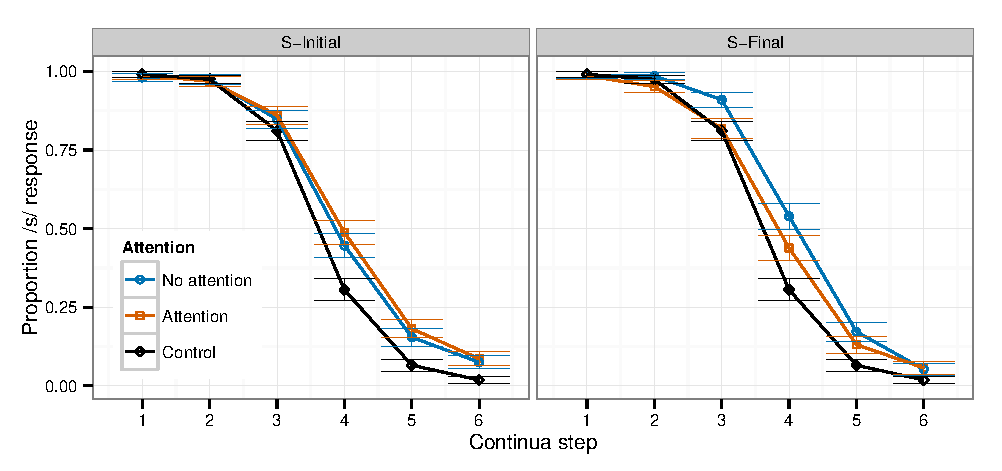
\includegraphics[width=\textwidth]{graphs/exp1_categresults}
\end{center}
\end{figure*}

There was a significant effect for the intercept ($\beta = 0.83, SE = 0.31, z = 2.6, p < 0.01$), indicating that participants categorized more of the continua as /s/ in general.  There was also a significant main effect of Step ($\beta = -2.10, SE = 0.20, z = -10.3, p < 0.01$), and a significant interaction between Exposure Type and Attention ($\beta = -0.93, SE = 0.43, z = -2.14, p = 0.03$).  There was a marginal main effect of Exposure Type ($\beta =0.58, SE = 0.30, z = 1.8, p = 0.06$).  

These results are shown in Figure~\ref{fig:exp1categ}.  
The solid lines show the control participants' categorization function across the 6 steps of the continua.  
The error bars show within-subject 95\% confidence intervals at each step.  
When exposed to ambiguous /s/ tokens in the first syllables of words, participants show a general expansion of the /s/ category, but no differences in behaviour if they are warned about ambiguous /s/ productions.  
However, when the exposure is to ambiguous /s/ tokens later in the words, we can see differences in behaviour beyond the general /s/ category expansion.  
Participants not warned of the speaker's ambiguous tokens categorized more of the continua as /s/ than those who were warned of the speaker's ambiguous /s/ productions.

\begin{figure*}[!ht]

\caption{Correlation of crossover point in categorization with the proportion of word responses to critical items containing an ambiguous /s/ token.}\label{fig:exp1xover}
\begin{center}
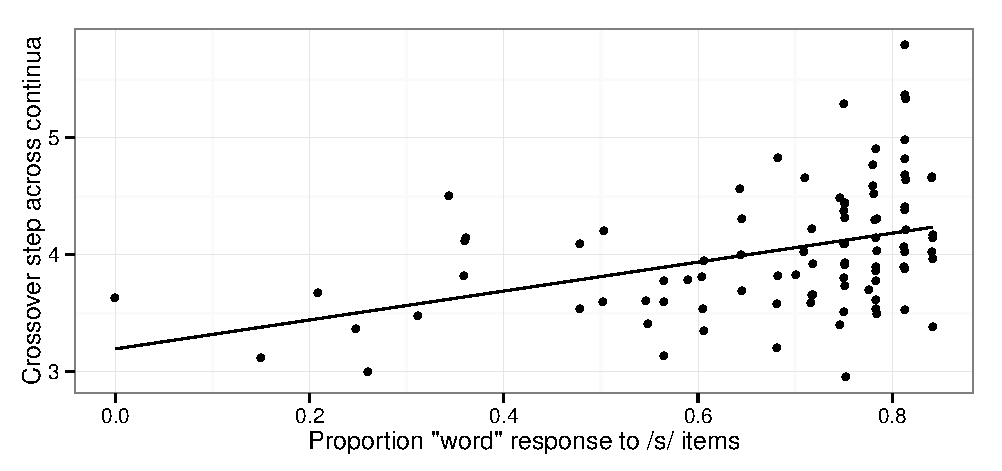
\includegraphics[width=\textwidth]{graphs/exp1_xoverwordresp}
\end{center}
\end{figure*}

As an individual predictor of participants' performance we took the proportion critical word endorsements and compared these values to the estimated cross-over points. 
The crossover point was determined from the Subject random effect in the logistic mixed effects model \citep{Kleber2011}. 
There was a significant positive correlation between a participant's tolerance for the ambiguous exposure items and their crossover point on the continua ($r = 0.39, t (90) = 4, p < 0.01$), shown in Figure~\ref{fig:exp1xover}.

An ANOVA with cross-over point as the independent variable and word endorsement rate, Exposure Type, Attention and their interactions, found only a main effect of word endorsement rate ($F(1,89) = 17.82, p < 0.01$), suggesting that listeners in different conditions were not affected differently from one another.


\subsection{Experiment 2}

\subsubsection{Exposure}

Trials with nonword stimuli and responses faster than 200 ms or slower than 2500 ms were excluded from analysis. 
Performance on the exposure task was high overall, with accuracy on filler trials averaging 92\%.  
An ANOVA of critical word endorsement rates revealed a marginal effect of Exposure Type ($F(1,92) = 3.86, p = 0.05$), with participants in the S-Final conditions having lower word endorsement rates (S-Final/Attention: mean = 56\%, sd = 30\%; S-Final/No Attention: mean = 52\%, sd = 25\%) than participants in the S-Initial conditions (S-Initial/Attention: mean = 68\%, sd = 25\%; S-Initial/No Attention: mean = 61\%, sd = 23\%).
A logistic mixed effects model with accuracy as the dependent variable was fit with fixed effects for trial type (Filler, S, SH), Attention (No Attention, Attention), Exposure Type (S-Initial, S-Final) and their interactions. 
The random effect structure was as maximally specified as possible with random effects for Subject and Word, and by-Subject random slopes for trial type and by-Word random slopes for Attention. 
The only fixed effect that was significant were a main effect of trial type for /s/ trials compared to filler trials ($\beta = -2.51, SE = 0.46, z = -5.35, p < 0.01$).

\subsubsection{Categorization}

Responses with reaction times less than 200 ms or greater than 2500 ms were excluded from analyses. 
Participants were excluded if their initial estimated cross over point for the continuum lay outside of the 6 steps presented (2 participants).  
A logistic mixed effects model was constructed with Subject and Continua as random effects and continua Step as random slopes, with 0 coded as a /\textesh/ response and 1 as a /s/ response.  Fixed effects for the model were Step, Exposure Type, Attention and their interactions.

\begin{figure*}[!ht]
\caption{Proportion /s/ response along the 6 step continua as a function of Exposure Type and Attention in Experiment 2.  Participants showed no significant differences across conditions. Error bars represent 95\% confidence intervals.}
\label{fig:exp2categ}
\begin{center}
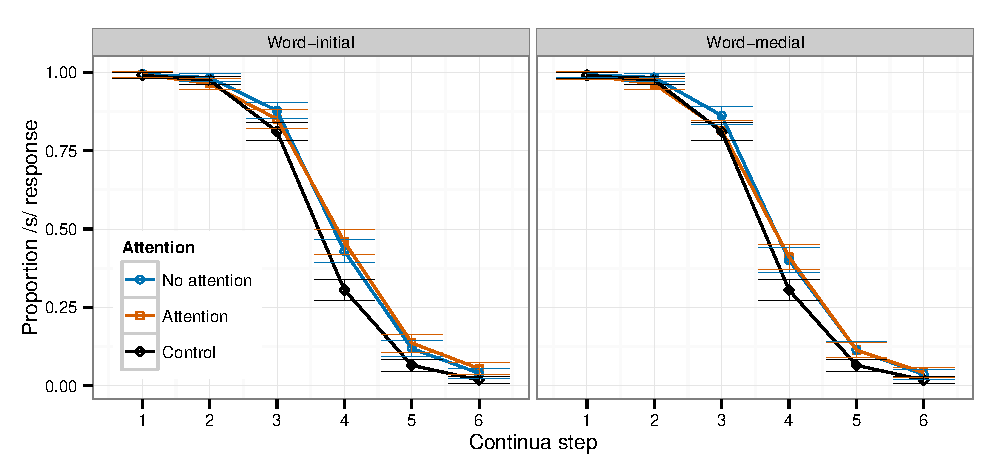
\includegraphics[width=\textwidth]{graphs/exp2_categresults}
\end{center}
\end{figure*}

There was a significant effect for the Intercept ($\beta = 1.01, SE = 0.38, z = 2.6, p < 0.01$), indicating that participants categorized more of the continua as /s/ in general.  There was also a significant main effect of Step ($\beta = -2.67, SE = 0.23, z = -11.2, p < 0.01$).  There were no other significant main effects or interactions, though an interaction between Step and Attention trended toward significant ($\beta = 0.35, SE = 0.21, z = 1.6, p = 0.09$).

\begin{figure*}[!ht]

\caption{Correlation of crossover point in categorization with the proportion of word responses to critical items containing an ambiguous /s/ token in Experiment 2.}\label{fig:exp2xover}
\begin{center}
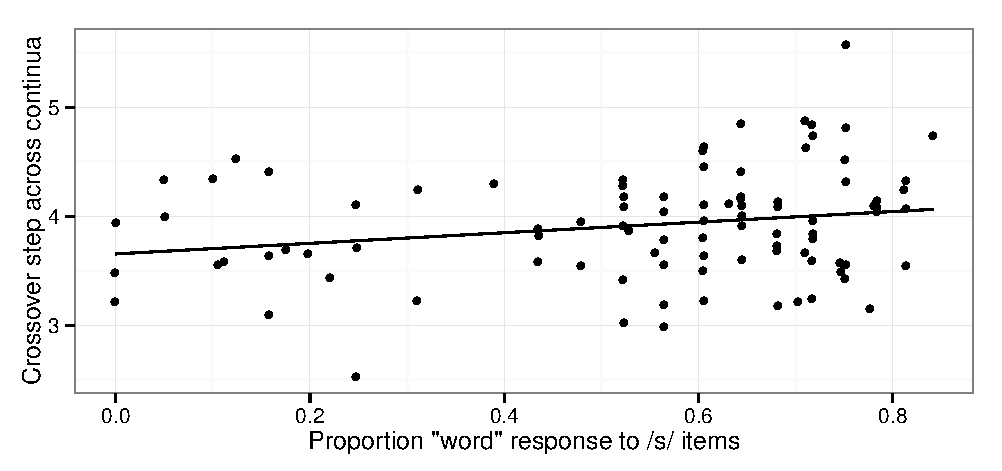
\includegraphics[width=\textwidth]{graphs/exp2_xoverwordresp}
\end{center}
\end{figure*}

As in Experiment 1,  the proportion critical word endorsements was calculated for each subject and assessed for correlation with participants' crossover points. There was a significant positive correlation between a participant's tolerance for the ambiguous exposure items and their crossover point on the continua ($r = 0.22, t (92) = 2.25, p = 0.02$), shown in Figure~\ref{fig:exp2xover}.  

\section{Grouped results across experiments}

To see what degree the stimuli used had an effect on perceptual learning, the data from Experiment 1 and Experiment 2 were pooled and analyzed identically as above, but with Experiment and its interactions as fixed effects.  In the logistic mixed effects model, there was significant main effects for Intercept ($\beta = 1.00, SE = 0.36, z = 2.7, p < 0.01$) and Step ($\beta = -2.64, SE = 0.21, z = -12.1, p < 0.01$), and a significant two-way interaction between Experiment and Step ($\beta = 0.51, SE = 0.20, z = 2.5, p = 0.01$), and a marginal four-way interaction between Step, Exposure Type, Attention and Experiment ($\beta = 0.73, SE = 0.42, z = 1.7, p = 0.08$).  These results can be seen in Figure~\ref{fig:exp12categ}.  The four-way interaction can be seen in S-Final/No Attention conditions across the two experiments, where Experiment 1 has a significant difference between the Attention and No Attention condition, but Experiment 1 does not.  The two-way interaction between Experiment and Step and the lack of a main effect for Experiment potentially suggests that while the category boundary was not significantly different across experiments, the slope of the categorization function was.

\begin{figure*}[!ht]
\caption{Proportion /s/ response along the 6 step continua as a function of Exposure Type and Attention in Experiment 1 and Experiment 2. Error bars represent 95\% confidence intervals.}
\label{fig:exp12categ}
\begin{center}
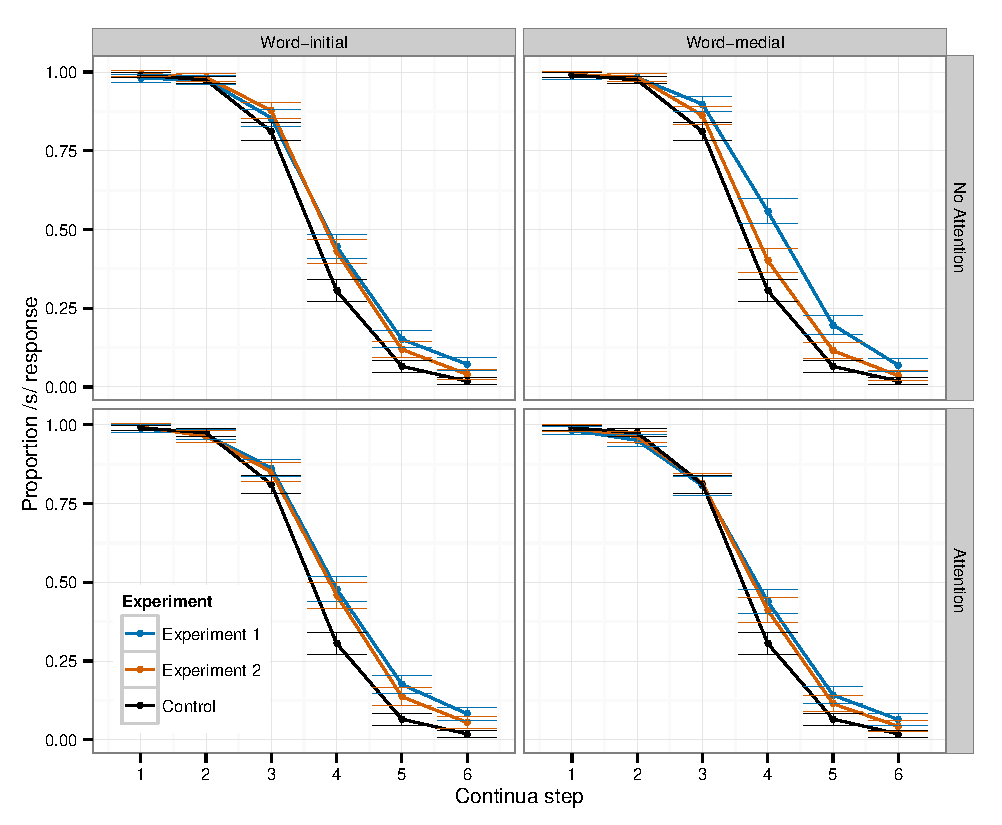
\includegraphics[width=\textwidth]{graphs/exp12_categresults}
\end{center}
\end{figure*}

To see if there was a difference with the Experiment 1 in how word endorsement rates affected crossover points, the data was pooled for the two experiments.  An ANOVA with cross-over point as the independent variable and word endorsement rate, Exposure Type, Attention, Experiment and their interactions, found a main effect of word endorsement rate ($F(1,185) = 21.82, p < 0.01$) and marginal interaction between word endorsement rates and Experiment ($F(1, 185) = 3.11, p = 0.07$).

\subsection{Experiment 3}

There's not much here at the moment...

\subsection{Exposure}

Performance in the task was high, with accuracy at ceiling.

\subsection{Categorization}



\begin{figure*}[!ht]
\caption{Proportion /s/ response along the 6 step continua as a function of Exposure Type and Attention in Experiment 3.  Error bars represent 95\% confidence intervals.}
\label{fig:exp3categ}
\begin{center}
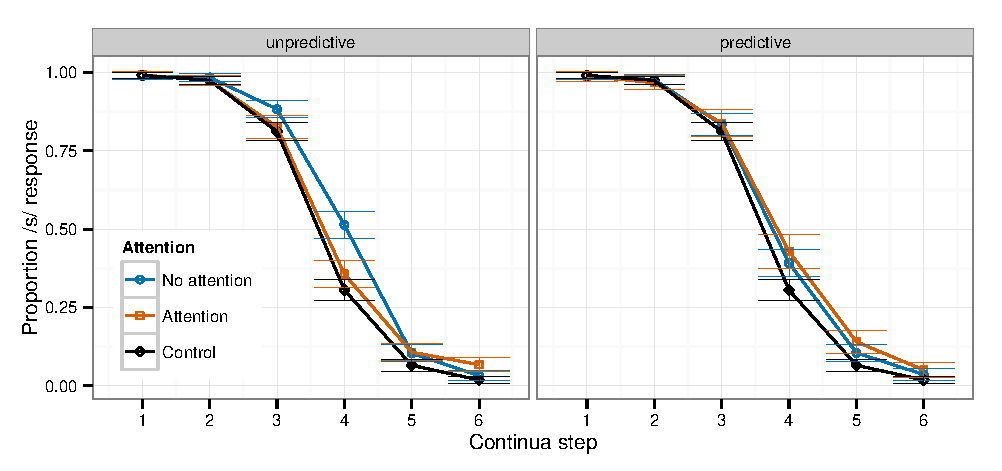
\includegraphics[width=\textwidth]{graphs/exp3_categresults}
\end{center}
\end{figure*}

\bibliographystyle{apalike}
\bibliography{biblio}

\end{document}
